\chapter{Project Context}

% ─────────────────────────────────────────────
\section*{Introduction}
\addcontentsline{toc}{section}{Introduction}
% ─────────────────────────────────────────────

\paragraph{}This chapter presents the professional and organizational context of this internship project. It begins with an introduction to Linedata Services, the host company, followed by a description of its Tunisian office. We then provide an overview of Longview, the front-office trade management platform, covering its main functions and the key financial entities that make up its data model. The rest of the chapter examines the test data preparation methods currently used by the quality assurance and development teams, highlighting their main limitations and practical challenges. Finally, we define the core problem that motivated this project and outline the structure of the remaining chapters.

% ─────────────────────────────────────────────
\section{Host Organization: Linedata}
% ─────────────────────────────────────────────

\begin{figure}[htbp]
\centering

\includegraphics[width=0.4\textwidth]{img/linedata_logo_square.png}
\caption{Logo of Linedata \cite{linedata_about}}
\label{fig:linedata}
\end{figure}

\paragraph{}Linedata Services S.A. was founded in 1998 and has grown into a major player in the financial technology industry. The company is headquartered in Neuilly-sur-Seine, France, and operates in more than twenty offices across Europe, North America, Asia, and Africa. As of 2024, Linedata employs over 1,100 people and serves around 700 clients in 50 countries, with annual revenues exceeding \texteuro{}183 million. The company is listed on Euronext Paris under the ticker symbol LIN \cite{linedata_about, linedata_revenue}.

\paragraph{}Linedata's main goal is to make financial technology more accessible and effective by offering software platforms, data management solutions, and professional services. Its products help financial institutions such as asset managers, hedge funds, and lending organizations improve their operational efficiency, flexibility, and regulatory compliance. The company's offerings are organized into two main business segments: Asset Management and Lending \& Leasing \cite{linedata_about}.

\begin{itemize}
\item \textbf{Asset Management:} End-to-end software solutions covering portfolio management, order and execution management (OMS/EMS), investment compliance, risk analytics, and fund administration. More than 63,000 financial professionals use Linedata's asset management products every day.
\item \textbf{Lending \& Leasing:} Complete solutions for lending institutions and leasing companies, covering origination, servicing, and portfolio management.
\end{itemize}

\paragraph{}Linedata's technology is built for cloud deployment and can scale horizontally. It uses an open architecture that can connect with third-party accounting systems, trading platforms, external data providers, and custodial interfaces. The company has also been progressively integrating artificial intelligence and machine learning into its data management and analytical workflows \cite{linedata_ai}.

% ─────────────────────────────────────────────
\subsection{Linedata Tunisia}
% ─────────────────────────────────────────────

\paragraph{}The Tunisian subsidiary of Linedata plays a central role in the company's research, development, and engineering activities. Located in Tunis, the office employs software engineers, quality assurance specialists and technical leads who are responsible for the development and maintenance of Linedata's core financial platforms, particularly the Longview system.

\begin{itemize}
\item \textbf{Address:} Immeuble Cléopâtre Center, Bloc B, Centre Urbain Nord, 1082 Tunis, Tunisia
\item \textbf{Phone:} +216 71 185 800
\end{itemize}

% ─────────────────────────────────────────────
\subsection{Organizational Structure and Internship Context}
% ─────────────────────────────────────────────

\paragraph{}Engineering work at Linedata Tunisia is divided into dedicated product teams that operate under the research and development department. The internship described in this report was carried out within the Longview development team.

\begin{figure}[htbp]
\centering
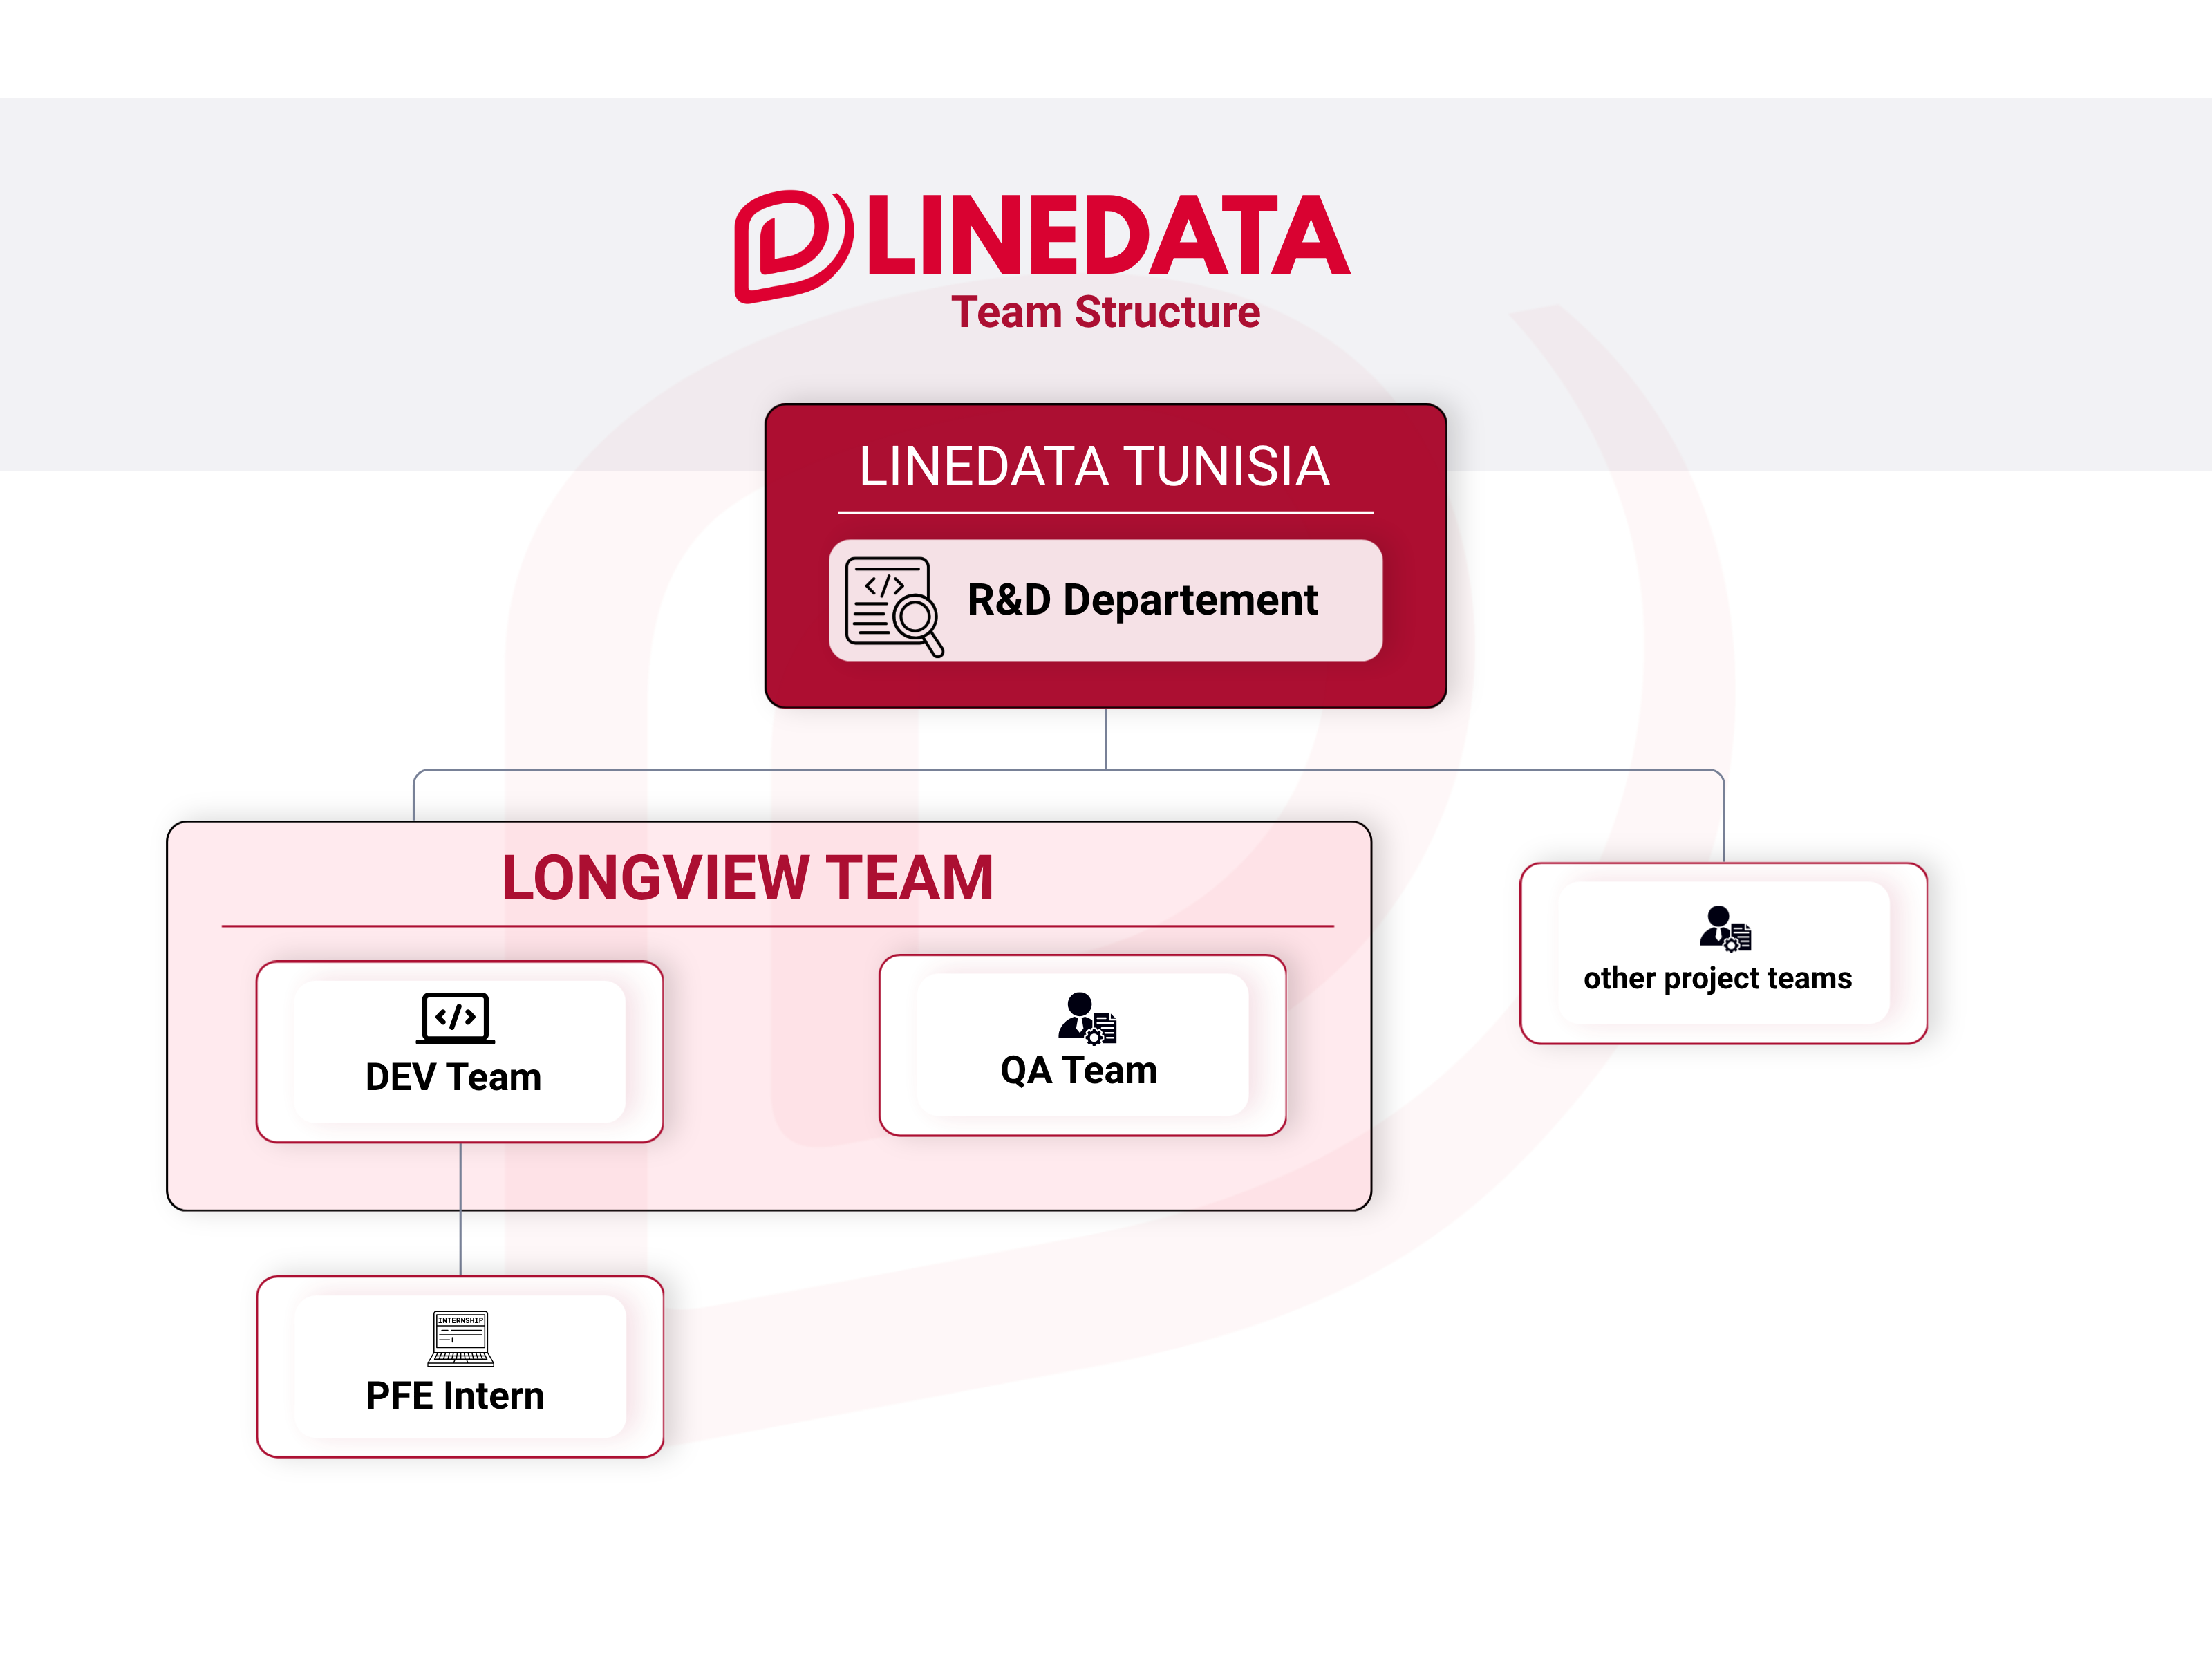
\includegraphics[width=0.82\textwidth]{img/orgchart.png}
\caption{Organizational structure of Linedata Tunisia and internship team placement}
\label{fig:orgchart}
\end{figure}

\paragraph{}The main goal of this internship was to design and build a configurable system that can generate valid test data for the Longview platform. This system was created to resolve the serious inefficiencies found in the existing manual test data preparation process.

% ─────────────────────────────────────────────
\section{Longview}
% ─────────────────────────────────────────────

\begin{figure}[htbp]
\centering
\includegraphics[width=0.5\textwidth]{img/longview_logo.png}
\caption{Linedata Longview, Front-Office Trade Order Management Platform \cite{longview_oms}}
\label{fig:longview}
\end{figure}

\paragraph{}Longview is an integrated, multi-tenant front-office trade order management platform built specifically for buy-side financial institutions. The platform supports the full investment lifecycle, including portfolio construction, compliance checks, order management, electronic trade execution, and post-trade settlement. Built on a relational SQL Server database, Longview supports continuous global trading operations and automated end-to-end processing. At the time of this project, the platform was at version 8.2 and continues to receive regular maintenance and improvements \cite{longview_oms}.

% ─────────────────────────────────────────────
\subsection{Core Financial Entities}
% ─────────────────────────────────────────────

\paragraph{}The Longview data model is built around a set of related financial entities that must maintain strict referential integrity and comply with business rule constraints. The platform's architecture is centered on several key entity types, including Accounts, Securities, Orders, Executions, and Positions.

\begin{itemize}
\item \textbf{Accounts:} Investment portfolios or client mandates, each identified by a unique account ID, linked to a base currency, a portfolio manager, and optional regulatory and compliance attributes.
\item \textbf{Securities:} Financial instruments across multiple asset classes, including equities and funds, fixed income instruments (bonds, money market securities, mortgage pass-throughs), futures, options, and FX forwards. Each type has its own required fields and valuation rules.
\item \textbf{Orders:} Buy or sell instructions created by portfolio managers, linked to specific accounts and securities, and subject to quantity, timing, and allocation constraints.
\item \textbf{Executions and Positions:} Trade confirmations produced when orders are filled, and the resulting inventory positions held by each account across its securities.
\end{itemize}

\paragraph{}The complex relationships and constraints between these entities make generating valid test data a challenging task. Any violation of referential integrity or business rules makes a dataset unusable and reduces the effectiveness of the quality assurance process.

% ─────────────────────────────────────────────
\section{Current Testing Procedure}
% ─────────────────────────────────────────────

\paragraph{}Ensuring the correctness and reliability of each Longview release requires a solid and continuous testing process. The quality assurance and development teams are responsible for validating new features, running regression tests, and confirming that existing functionality is preserved as the platform evolves. This process depends on having relevant, varied, and realistic test datasets.

% ─────────────────────────────────────────────
\subsection{Manual Test Data Preparation}
% ─────────────────────────────────────────────

\paragraph{}Currently, test data is generated through mostly manual procedures. Quality assurance engineers and developers write SQL scripts by hand and execute them against the Longview SQL Server database using INSERT, TRUNCATE, and IDENTITY\_INSERT statements, as well as stored procedure calls. For each test scenario, team members must identify the relevant database tables, manually build valid records that satisfy all primary and foreign key relationships, and verify that the data follows Longview's business rules. This process requires a thorough understanding of both the SQL Server schema and financial domain logic.

% ─────────────────────────────────────────────
\subsection{Limitations of the Current Approach}
% ─────────────────────────────────────────────

\paragraph{}The manual approach has several important limitations that reduce the efficiency, coverage, and reliability of the quality assurance process:

\begin{itemize}
\item \textbf{Time-consuming:} Building a complete dataset across multiple dependent tables can take hours for complex scenarios, such as full trade lifecycles involving group orders, multi-account allocations, and broker tickets.
\item \textbf{Error-prone:} Human mistakes such as mismatched foreign keys, execution quantities exceeding the parent order quantity, or missing price records frequently cause test failures that are unrelated to the feature being tested, leading to wasted debugging time.
\item \textbf{Lack of reproducibility:} Test data is created on an ad hoc basis and is not stored in a structured, version-controlled format, making it difficult to reproduce, share, or reuse across regression cycles.
\item \textbf{Confidentiality constraints:} Production data cannot be used for testing due to strict confidentiality agreements and regulatory requirements, so teams must rely entirely on artificially constructed datasets.
\end{itemize}

\begin{figure}[htbp]
\centering
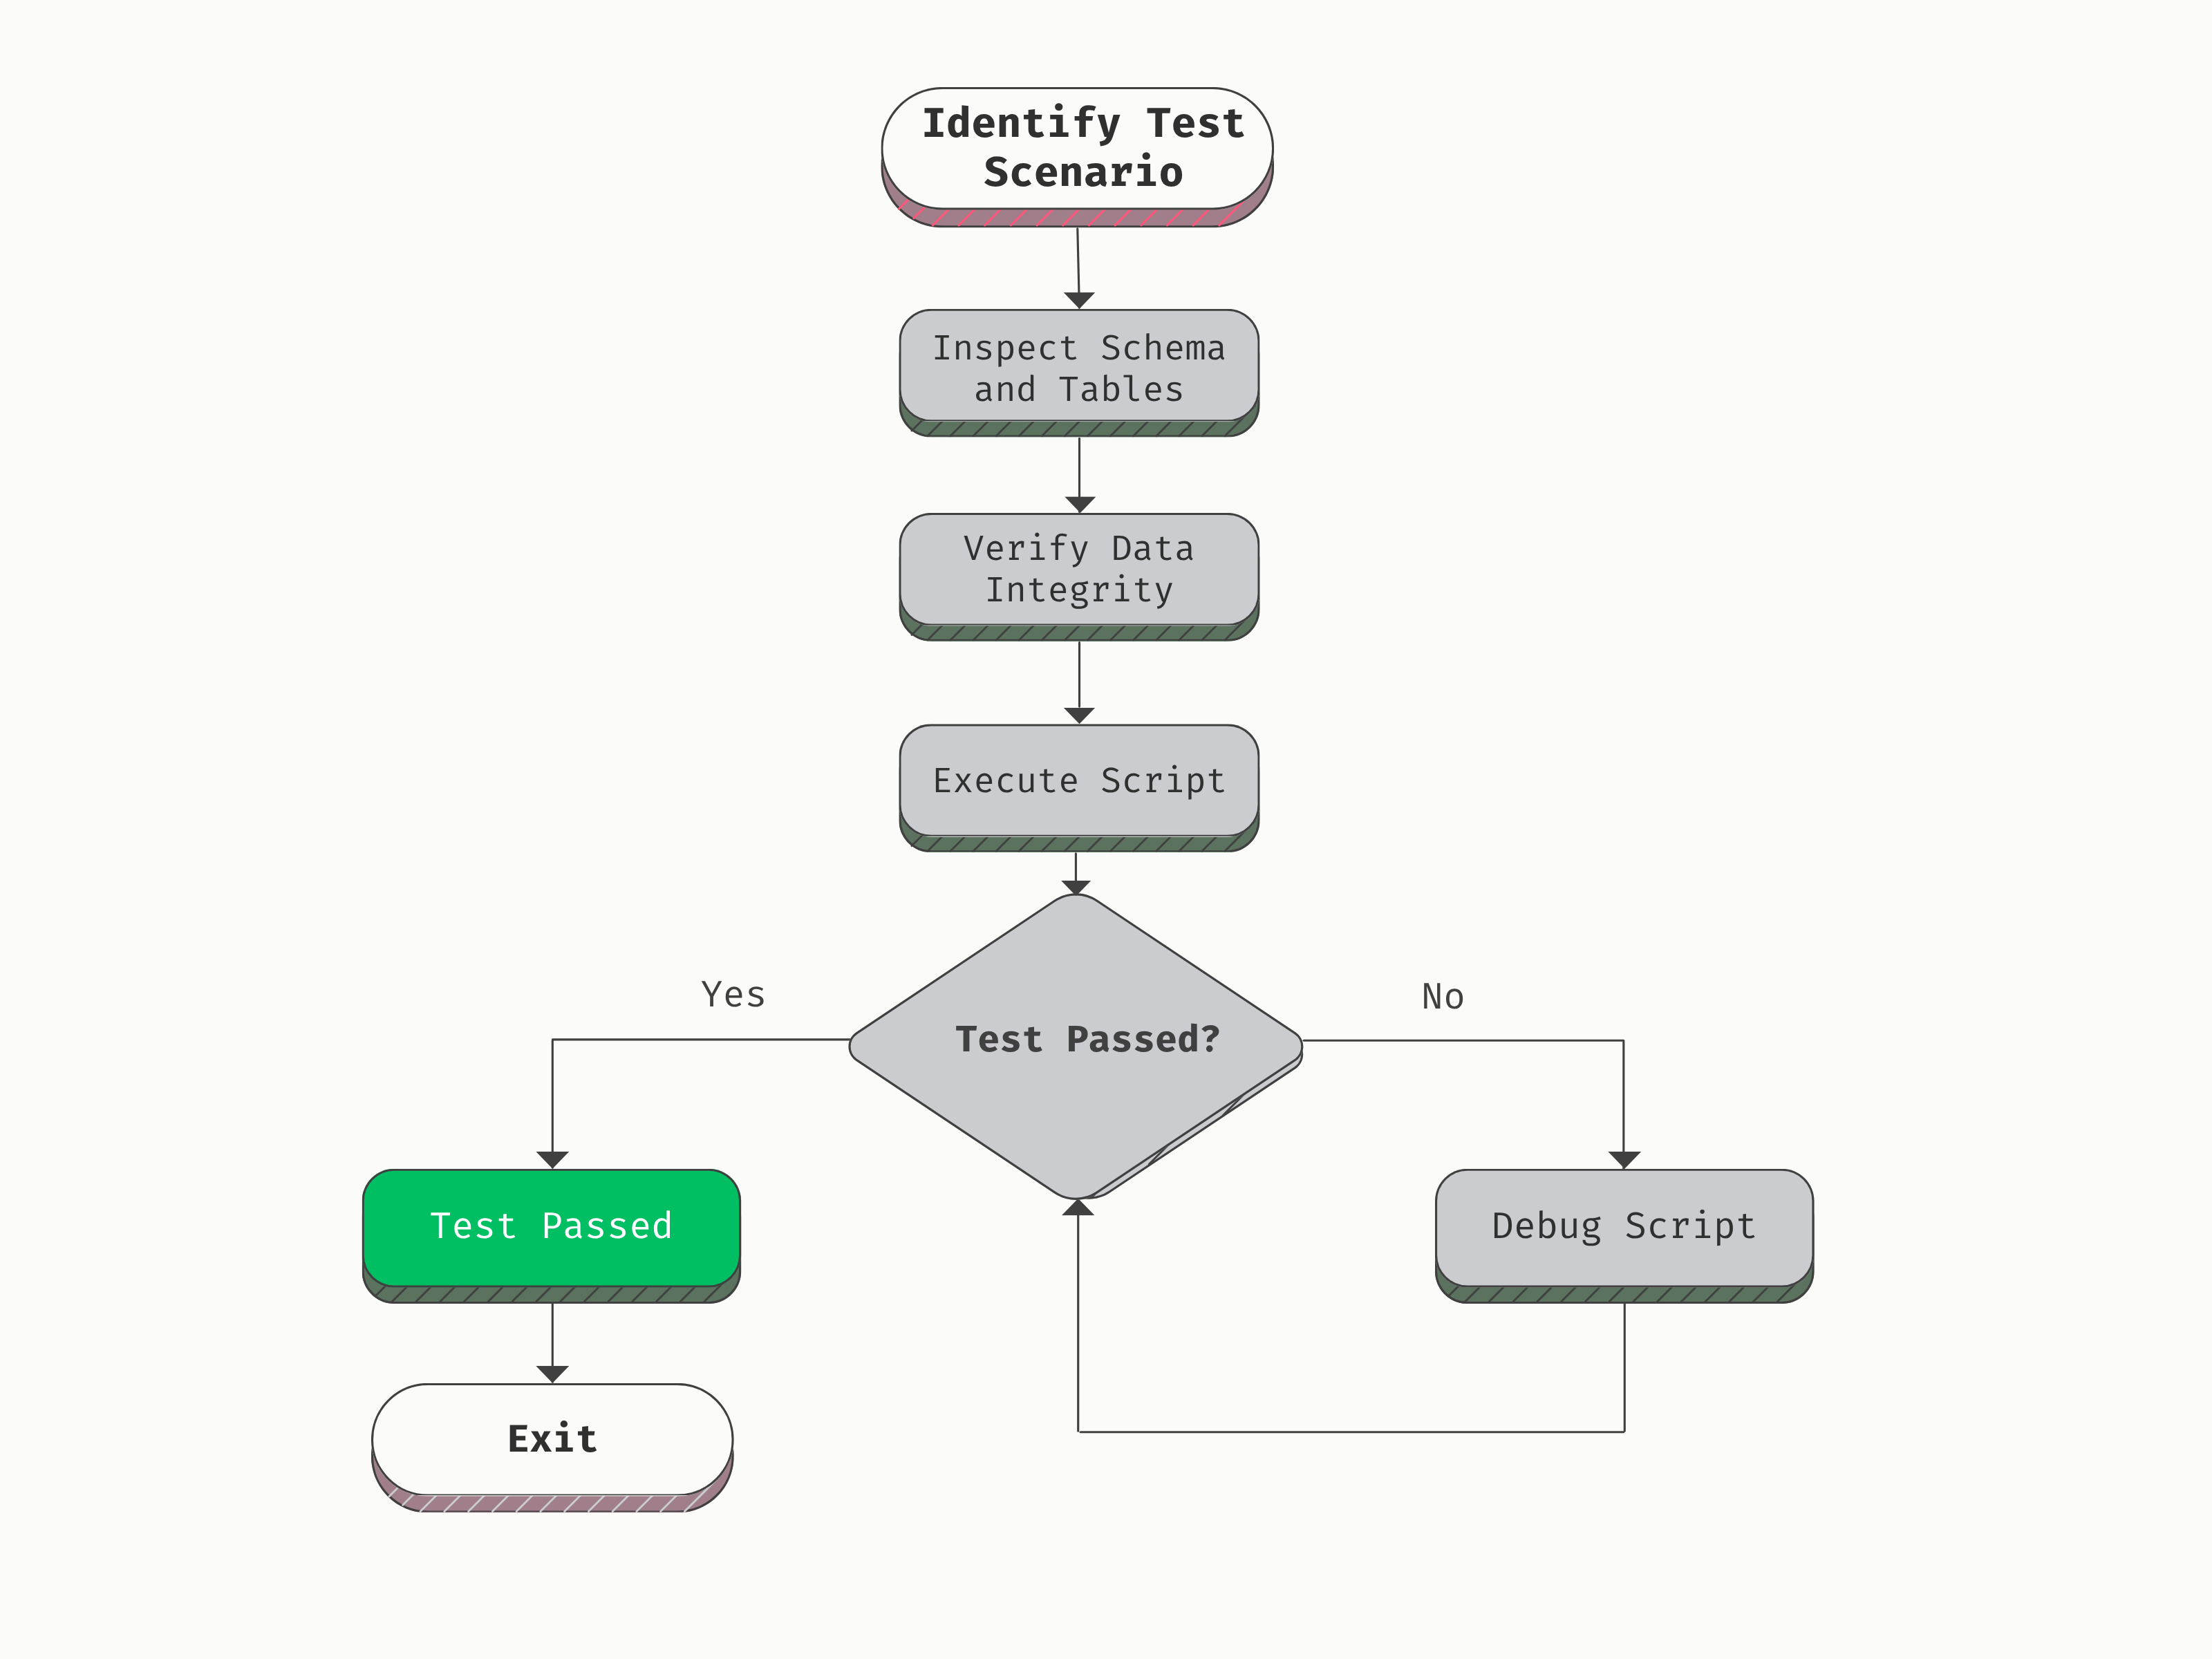
\includegraphics[width=0.85\textwidth]{img/current-process.png}
\caption{Current manual test data creation workflow at Linedata}
\label{fig:current-process}
\end{figure}

% ─────────────────────────────────────────────
\section{Problem Statement}
% ─────────────────────────────────────────────

\paragraph{}These limitations together point to a significant gap in Linedata's testing infrastructure. As the Longview platform expands to support a wider range of financial instrument types and regulatory frameworks, the need for varied and quickly deployable test data grows accordingly. The current manual approach is not able to meet these growing demands.

\paragraph{}This situation leads to the central problem statement of this project: \textit{How can Linedata's development and quality assurance teams be provided with an automated, configurable, and domain-aware tool that can generate realistic, coherent, and SQL-compatible test data for the Longview platform, while correctly enforcing the complex relationships between entities and the financial business rules that govern its data model?}

\paragraph{}This question breaks down into three core challenges:

\begin{itemize}
\item \textbf{Financial data consistency:} Generating valid test data requires enforcing business rules across dozens of interdependent tables at the same time. Any violation makes the dataset unusable.

\item \textbf{Dual-mode operation:} The tool must work in two distinct modes. In \textit{standalone mode}, it generates fully synthetic data without needing any database connection. In \textit{connected mode}, it establishes a read-only connection to an existing Longview SQL Server instance, retrieves real reference data (securities, accounts, models), and generates additional records that are consistent with the existing database state.

\item \textbf{Configurability and usability:} Test engineers must be able to specify data volume, instrument types, date ranges, and other parameters through an easy-to-use web interface, save and reuse generation configurations through a local library, and access the tool without requiring deep technical knowledge.
\end{itemize}

\paragraph{}Addressing these challenges required designing and building a full-stack web application that includes modular generation services for each financial entity, read-only SQL Server integration for connected operation, a local configuration library for saving and reusing generation presets, and optional Large Language Model integration for improved data realism. The system remains fully functional even when LLM support is unavailable. This is the core system described and developed throughout the rest of this report.

% ─────────────────────────────────────────────
\section{Proposed Solution}
% ─────────────────────────────────────────────

\paragraph{}To address the identified challenges, a configurable test data generation system named \textbf{Longview Test Data Generator} has been designed and implemented. The system operates in two complementary modes: \textit{standalone mode} generates fully synthetic test data without requiring any database connection, while \textit{connected mode} integrates with an existing Longview SQL Server instance in read-only mode to retrieve reference data and generate supplementary records that remain consistent with the production environment. The application also includes a configuration library that allows users to save, reload, and reuse generation settings across testing sessions. Through these features, the tool provides QA engineers and developers with a flexible, automated approach to generating valid, realistic, and reproducible test datasets on demand.

% ─────────────────────────────────────────────
\section*{Conclusion}
\addcontentsline{toc}{section}{Conclusion}
% ─────────────────────────────────────────────

\paragraph{}This chapter has established the professional and technical context for this project. We introduced Linedata and its Tunisian office as the host organization, and identified the Longview development team as the internship setting. We presented the Longview platform and described the core financial entities that make up its data model. The chapter reviewed the current manual test data creation process and identified its main weaknesses in terms of efficiency, error management, and time consumption. Finally, we defined the central problem statement: the need for an automated, domain-aware, and configurable test data generation system for Longview that supports both standalone and connected operation modes. The following chapter presents the requirements analysis, the adopted development methodology, the global architecture, and the sprint planning of the project.
